\documentclass{beamer}
\usepackage[utf8]{inputenc}
\usepackage[spanish]{babel}
\usepackage{hyperref}
\usepackage{verbatim}
\usepackage{listings}

\setbeamercovered{invisible}
\usetheme{Frankfurt}
\usefonttheme{serif}

% Configurar los listings (Códigos)
\renewcommand{\lstlistingname}{Código}
\lstset{
	language=C++,               % Lenguaje
	basicstyle=\ttfamily\footnotesize,  % Tipo de fuente
	keywordstyle=\color{blue},  % Color de palabras clave
	stringstyle=\color{red},    % Color de strings
	commentstyle=\color{gray},  % Color de comentarios
	showstringspaces=false,     % No muestrar el _ cuando el string tiene espacios
	breaklines = true,          % Partir las líneas largas
	breakatwhitespace=true,	    % Partir las líneas en un espacio
	numbers=left,				% Numerar las líneas a la izq
	numberstyle=\tiny,			% Poner los números de las líneas pequeños
	numberblanklines=true,      % Numerar las líneas en blanco
	columns=fullflexible,       % No perder el formato al dejar los espacios
	keepspaces=true,   			% Dejar los espacios insertados
	frame=tb,					% Poner el recuadro
}


\title{Semillero de Programación}
\subtitle{Problemas con DFS, BFS, Componentes Fuertemente Conexas y Ordenamiento Topológico}
\author{Ana Echavarría \and Juan Francisco Cardona}

\institute{Universidad EAFIT}
\date{1 - 8 marzo de 2013}

\begin{document}

\begin{frame}
	\titlepage
\end{frame}

\begin{frame}
	\frametitle{Contenido}
	\tableofcontents
\end{frame}

\section{Bicoloring}
	\begin{frame}
		\frametitle{Problema 10004 - Bicoloring}
		\begin{block}{Problema}
			Verificar si un grafo es bipartito, es decir, si se pueden usar dos colores para pintar todos los nodos de manera que dos nodos vecinos no tengan el mismo color
		\end{block}
	\end{frame}
	
	\begin{frame}
		\frametitle{¿Qué técnica usar?}
		\begin{alertblock}{Pregunta}
				\begin{itemize}
					\item ¿Cómo hago para verificar que el grafo sea bipartito? \pause
						\begin{itemize}
							\item Pinto el primer nodo de un color y todos sus vecinos de otro color y repito el proceso con los vecinos. \pause
						\end{itemize}
					\item ¿Qué pasa si tengo que pintar un nodo que ya pinté antes? \pause
						\begin{itemize}
							\item Si el color con el que lo tengo que pintar es el mismo que tiene no pasa nada, si no es así el grafo no es bipartito.
						\end{itemize}
					\item ¿Qué técnica puedo usar para pintar cada nodo y luego sus vecinos? \pause
						\begin{itemize}
							\item Se pueden usar BFS y DFS.
						\end{itemize}
				\end{itemize}
		\end{alertblock}
	\end{frame}
	
	\begin{frame}[fragile]
		\frametitle{Solución}
		\begin{lstlisting}
			int main(){
			   int n, m;
			   while (cin >> n){
			      if (n == 0) break;
			      for (int i = 0; i < n; ++i){
			         g[i].clear();
			         color[i] = -1;
			      }
			      cin >> m;
			      for (int i = 0; i < m; ++i){
			         int u, v;
			         cin >> u >> v;
			         g[u].push_back(v);
			         g[v].push_back(u);
			      }
			      if (dfs(0, 0)) puts("BICOLORABLE.");
			      else puts("NOT BICOLORABLE.");
			   }
			    return 0;
			}
		\end{lstlisting}
	\end{frame}
	
	\begin{frame}[fragile]
		\frametitle{Solución usando DFS}
		\begin{lstlisting}
			const int MAXN = 205;
			vector <int> g[MAXN];
			int color[MAXN];

			bool dfs(int u, int paint){
			   color[u] = paint;
			   for (int i = 0; i < g[u].size(); ++i){
			      int v = g[u][i];
			      bool possible;
			      if (color[v] == -1) possible = dfs(v, 1 - paint);
			      else possible = (color[v] == (1 - paint));
			      if (!possible) return false;
			   }
			   return true;
			}
		\end{lstlisting}
	\end{frame}
	
	\begin{frame}[fragile]
		\frametitle{Solución usando BFS}
		\begin{lstlisting}
		bool bfs(int s){
		   queue <int> q;
		   q.push(s);
		   color[s] = 0;
		   while (q.size() > 0){
		      int u = q.front(); q.pop();
		      for (int i = 0; i < g[u].size(); ++i){
		         int v = g[u][i];
		         if (color[v] == color[u]) return false;

		         if (color[v] == -1){
		            color[v] = 1 - color[u];
		            q.push(v);
		         }
		      }
		   }
		   return true;
		}
		\end{lstlisting}
	\end{frame}
	

\section{Playing with Wheels}
	\begin{frame}
		\frametitle{Problema 10067 - Playing with Wheels}
		Se tiene una caja fuerte con 4 ruedas que indican cada una un número. Cada rueda tiene dos botones, uno mueve la rueda a la derecha (aumenta el número mostrado y si es 9 cambia al 0) y el otro mueve la rueda a la izquierda (disminuye el número mostrado y si es 0 cambia al 9).
		\begin{center} 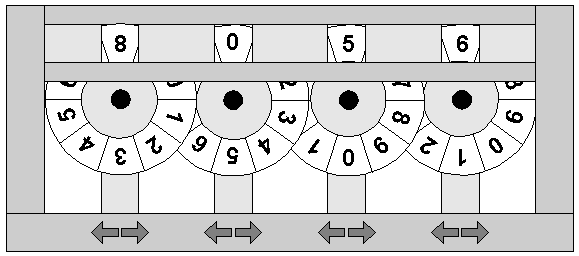
\includegraphics[height = 0.4\textheight]{wheels.png} \end{center}
	\end{frame}
	
	\begin{frame}
		\frametitle{Problema}
		\begin{itemize}
			\item Se sabe cuál es la configuración inicial de las ruedas y cuál es la configuración final que abre la caja fuerte. Sin embargo, hay un conjunto de configuraciones prohibidas que no se pueden activar.\\
			\item El problema es hallar el \textbf{mínimo número de movimientos de las ruedas que hay que hacer para llegar de la configuración inicial a la final sin pasar por ninguna de las configuraciones prohibidas.}
		\end{itemize}
	\end{frame}
	
	\begin{frame}
		\frametitle{¿Qué técnica usar?}
		\begin{alertblock}{Preguntas}
			\begin{enumerate}
				\item ¿El problema se puede expresar como un problema de grafos? \pause
				\item ¿Cuáles serían los nodos? \pause
				\item ¿Cuándo se forma una arista? (¿cuándo se unen dos nodos?) \pause
				\item ¿Cuántos nodos hay? \pause
				\item ¿Cuántas aristas hay? \pause
				\item ¿El grafo cambia con cada caso de prueba o es independiente de los casos de prueba? \pause
				\item ¿Cómo hallo el mínimo número de movimientos para llegar de un nodo al otro?
			\end{enumerate}
		\end{alertblock}
	\end{frame}
	
	\begin{frame}
		\frametitle{Representación del grafo}
		Cada nodo del grafo es un vector enteros de 4 posiciones, sin embargo en el algoritmo asumimos que los nodos son número enteros. ¿Hay alguna forma de representar estos nodos como números? ¿Si la hay, pueden dos nodos tener la misma representación?
	\end{frame}
	
	\begin{frame}[fragile]
		\frametitle{Creación del grafo}
		\begin{lstlisting}
			const int MAXN = 10005;
			// Find neighbour of node u if you move wheel d in direction dir
			int find_neighbour(int u, int d, int dir){
			   vector <int> a(4);
			   for (int i = 0; i < 4; ++i){
			      a[i] = u % 10;
			      u /= 10;
			   }
			   a[d] = (a[d] + 10 + dir) % 10;

			   int ans = 0;
			   for (int i = 3; i >= 0; --i){
			      ans *= 10; ans += a[i];
			   }
			   return ans;
			}
		\end{lstlisting}
	\end{frame}
	
	\begin{frame}[fragile]
		\frametitle{Creación del grafo y lectura números}
		\begin{lstlisting}
			vector <int> g[MAXN];
			void make_graph(){ // Create out edges for all nodes
			   for (int i = 0; i <= 9999; ++i){
			      for (int d = 0; d < 4; ++d){
			         g[i].push_back(find_neighbour(i, d, -1)); // Move left
			         g[i].push_back(find_neighbour(i, d, +1)); // Move right
			      }
			   }
			}
		\end{lstlisting}
		
		\begin{lstlisting}
			int get_num(){ // Read nodes and convert them to an integer
			   int ans = 0;
			   for (int i = 0; i < 4; ++i){
			      int d; cin >> d;
			      ans = ans * 10 + d;
			   }
			   return ans;
			}
		\end{lstlisting}
	\end{frame}
	
	\begin{frame}[fragile]
		\frametitle{Lectura de los datos}
		\begin{lstlisting}
			bool forbidden[MAXN]; // The forbidden edges
			int d[MAXN];            // The distance for start vertex

			int main(){
			   make_graph();        // Create the graph
			   int cases; cin >> cases;
			   while (cases--){
			      for (int i = 0; i < MAXN; ++i) forbidden[i] = false;
			      int s = get_num(); // Read start vertex
			      int t = get_num(); // Read end vertex

			      int n; cin >> n;   // Read all forbidden vertices
			      while (n--) forbidden[get_num()] = true;
		
			      bfs(s);               // Call bfs from the start vertex
			      cout << d[t] << endl; // Output distance to end vertex
			   }
			   return 0;
			}
		\end{lstlisting}
	\end{frame}
	
	\begin{frame}[fragile]
		\frametitle{BFS}
		\begin{lstlisting}
			void bfs(int s){
			   for (int i = 0; i < MAXN; ++i) d[i] = -1;
			   queue <int> q;
			   q.push(s);
			   d[s] = 0;
			   while (q.size() > 0){
			      int cur = q.front(); q.pop();
			      for (int i = 0; i < g[cur].size(); ++i){
			         int next = g[cur][i];
			         // If not seen before and not forbidden add to queue
			         if (!forbidden[next] and d[next] == -1){ 
			            d[next] = d[cur] + 1;
			            q.push(next);
			         }
			      }
			   }
			}
		\end{lstlisting}
	\end{frame}

\section{Ordenamiento Topológico}
	\begin{frame}
		\frametitle{DAG}
		\begin{block}{DAG}
			Un DAG (Directed Acyclic Graph) es un grafo dirigido que no tiene ciclos.
		\end{block}
		\begin{center} 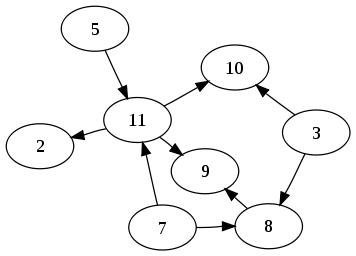
\includegraphics[height = 0.4\textheight]{DAG.png} \end{center}
	\end{frame}
	
	\begin{frame}
		\frametitle{Ordenamiento Topológico}
		\begin{block}{Ordenamiento Topológico}
			Un ordenamiento topológico o topological sort de un DAG $G = (V, E)$ es un ordenamiento lineal de sus nodos $V$ de tal forma que si $(u, v) \in E$ entonces $u$ aparece antes que $v$ en el ordenamiento.\\
			Este ordenamiento se puede ver como una forma de poner todos los nodos en una línea recta y que las aristas vayan todas de izquierda a derecha.
		\end{block}
	\end{frame}
	
	\begin{frame}
		\frametitle{Ejemplo}
		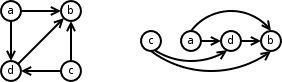
\includegraphics[width = 0.95\textwidth]{toposort.png}
	\end{frame}
	
	\begin{frame}
		\frametitle{Algoritmo}
		\begin{enumerate}
			\item Hacer un DFS con el grafo
			\item Cuando marco un nodo como negro, lo inserto a un vector
			\item Reversar el orden de los elementos del vector
			\item El vector contiene un ordenamiento topológico del grafo
		\end{enumerate}
	\end{frame}
	
	\begin{frame}[fragile]
		\frametitle{Algoritmo}
		\begin{lstlisting}
			vector <int> g[MAXN];
			bool seen[MAXN];
			vector <int> topo_sort;

			void dfs(int u){
			   seen[u] = true;
			   for (int i = 0; i < g[u].size(); ++i){
			      int v = g[u][i];
			      if (!seen[v]) dfs(v);
			   }
			   topo_sort.push_back(u); // Agregar el nodo al vector
			}
			int main(){
			   // Build graph: n = verices 
			   topo_sort.clear();
			   for (int i = 0; i < n; ++i) seen[i] = false;   
			   for (int i = 0; i < n; ++i) if (!seen[i]) dfs(i);  
			   reverse(topo_sort.begin(), topo_sort.end());
			   return 0;
			}
		\end{lstlisting}
	\end{frame}
	
	\begin{frame}
		\frametitle{Ejemplo}
		\begin{center} 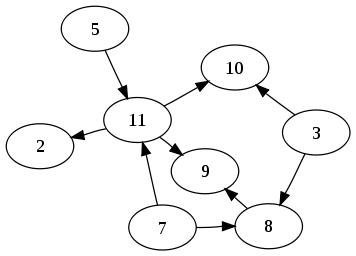
\includegraphics[height = 0.7\textheight]{DAG.png} \end{center}
	\end{frame}
	
	\begin{frame}
		\frametitle{¿Por qué funciona?}
		\begin{itemize}
			\item Cuando meto un nodo a la lista, es porque ya procesé todos sus vecinos.
			\item Si ya procesé todos sus vecinos, ellos ya están en la lista.
			\item Cuando meto un nodo a la lista, todos sus vecinos ya están antes que él en la lista, entonces en el ordenamiento van a quedar después de él.
			\item En conclusión, en el ordenamiento que generamos, los vecinos de cada nodo van a estar después de él por lo que es un ordenamiento topológico.
		\end{itemize}
	\end{frame}
	
	\begin{frame}
		\frametitle{Complejidad}
		\begin{block}{Complejidad}
			Hacer el ordenamiento topológico toma $O(V+E)$ para el dfs y $O(V)$ para reversar la lista. En total la complejidad es $O(V+E)$.
		\end{block}
	\end{frame}


\section{Componentes Fuertemente Conexas}
	\begin{frame}
		\frametitle{Componentes Fuertemente Conexas}
		\begin{block}{SCC}
			Dado un grafo dirigido $G = (V, E)$, un componente fuertemente conexa o strongly connected component (SCC) de $G$ es un subconjunto $C$ de nodos que cumple que para cada pareja $u, v \in C$ existe un camino de $u$ a $v$ y de $v$ a $u$ y que $C$ es lo más grande posible. 
		\end{block}
		\begin{center} 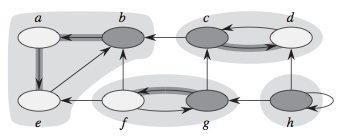
\includegraphics[height = 0.3\textheight]{scc.png} \end{center}
	\end{frame}
	
	\begin{frame}
		\frametitle{Algoritmo}
		\begin{enumerate}
			\item Crear el grafo $G$ y el grafo $G_{rev}$ que es el mismo que $G$ pero con las aristas invertidas.
			\item Hacer DFS en el grafo G y generar su ``ordenamiento topológico'' (incluir un nodo a la lista solo cuando haya visto todos los nodos alcanzables desde él.)
			\item Hacer un DFS en el grafo reversado $G_{rev}$ pero hacer las llamadas en el orden del ``ordenamiento topológico''.
			\item Cada llamado a este último DFS halla una componente fuertemente conexa.
		\end{enumerate}
	\end{frame}
	
	\begin{frame}
		\frametitle{Ejemplo}
		\begin{center} 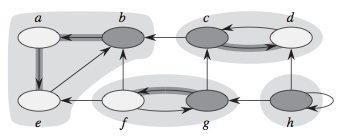
\includegraphics[height = 0.5\textheight]{scc.png} \end{center}
	\end{frame}
	
	\begin{frame}[allowframebreaks]
		\frametitle{¿Por qué funciona?}
		\begin{enumerate}
			\item Las componentes fuertemente conexas de $G$ son las mismas que las de $G_{rev}$.
			\item Si comprimo los nodos de una misma componente en un solo nodo, quedo con un DAG.
			\item Si tengo dos componentes distintas $C_1$ y $C_2$ de manera que haya una arista de un nodo de $C_1$ a un nodo de $C_2$, entonces todos los nodos de $C_1$ van a quedar después que los nodos de $C_2$ en el ``ordenamiento topológico'' que se hace con el primer DFS.
			\framebreak
			\item Los nodos que quedan de primeros en el ``ordenamiento topológico'' son los nodos de una componente $C$ a la cual no llega ninguna arista.
			\item En el grafo $G_{rev}$, de la componente $C$ no sale ninguna arista.
			\item Cuando llamo el segundo DFS lo hago desde $C$ y sólo descubro los elementos de $C$.
			\item Cuando llamo el segundo DFS desde otro nodo este puede no tener aristas salientes o tener aristas salientes a $C$ pero como ya descubrí todo en $C$ sólo voy a descubrir lo que hay en la componente de ese nodo
		\end{enumerate}
	\end{frame}

\section{Dominos}
	\begin{frame}
		\frametitle{Problema 11504 - Dominos}
		\begin{block}{Problema}
			Hallar el mínimo número de dominos que hay que derribar a mano para que todos los dominos se derriben.
		\end{block}
	\end{frame}
	
	\begin{frame}
		\frametitle{Ideas}
		\begin{alertblock}{Ideas}
			\begin{itemize}
				\item ¿Qué pasa con las cadenas de dominos que forman un ciclo? ¿Cuántos necesito máximo para derribarlas? \pause
				\item ¿Puedo entonces considerar los ciclos como un sólo dominó? ¿Qué algoritmo estoy utilizando? \pause
				\item ¿En el grafo que se forma cuando uno los elementos de una misma componentes cuántos dominos tengo que derribar?
			\end{itemize}
		\end{alertblock}
	\end{frame}
	
	\begin{frame}
		\frametitle{Solución}
		\begin{enumerate}
			\item Crear el grafo dirigido y su grafo invertido
			\item Hallar la componente fuertemente conexa de cada nodo
			\item Hallar cuantas aristas llegan a cada componente conexa
			\item Contar cuantas componentes hay a las cuales no lleguen aristas
		\end{enumerate}
	\end{frame}
	
	\begin{frame}[fragile]
		\frametitle{Variables globales}
		\begin{lstlisting}
			// El maximo numero de dominos
			const int MAXN = 100005; 
			// El grafo
			vector <int> g[MAXN];
			// El grafo reversado    
			vector <int> grev[MAXN];
			// El "ordenamiento topologico" del grafo G 
			vector <int> topo_sort;  
			// La componente fuertemente conexa a la que pertenece cada nodo
			int scc[MAXN];  
			// El arreglo de visitado para el primer DFS         
			bool seen[MAXN];
			 // El numero de aristas entrantes a cada componente         
			int in[MAXN];           
		\end{lstlisting}
	\end{frame}
	
	\begin{frame}[fragile]
		\frametitle{DFS}
		\begin{lstlisting}
			// DFS donde se halla el ordenamiento
			void dfs1(int u){ 
			   seen[u] = true;
			   for (int i = 0; i < g[u].size(); ++i){
			      int v = g[u][i];
			      if (!seen[v]) dfs1(v);
			   }
			   topo_sort.push_back(u);
			}
			// DFS donde se hallan las componentes
			void dfs2(int u, int comp){ 
			   scc[u] = comp;
			   for (int i = 0; i < grev[u].size(); ++i){
			      int v = grev[u][i];
			      if (scc[v] == -1) dfs2(v, comp);
			   }
			}
		\end{lstlisting}
	\end{frame}
	
	\begin{frame}[fragile, allowframebreaks]
		\frametitle{Main}
		\begin{lstlisting}
			int main(){
			   int cases; cin >> cases;
			   while (cases--){
			      int n, m;
			      cin >> n >> m;
			
			      // Limpiar las variables entre caso y caso
			      for (int i = 0; i <= n; ++i){
			         g[i].clear();
			         grev[i].clear();
			         topo_sort.clear();
			         scc[i] = -1;
			         seen[i] = false;
			         in[i] = 0;
			      }
			
			
			
			      // Crear el grafo y el grafo reversado
			      for (int i = 0; i < m; ++i){
			         int u, v; cin >> u >> v;
			         u--; v--;
			         g[u].push_back(v);
			         grev[v].push_back(u);
			      }
			
			      // Llamar el primer dfs
			      for (int i = 0; i < n; ++i){
			         if (!seen[i]) dfs1(i);
			      }
			      reverse(topo_sort.begin(), topo_sort.end()); 
			      // Llamar el segundo dfs
			      int comp = 0;
			      for (int i = 0; i < n; ++i){
			         int u = topo_sort[i];
			         if (scc[u] == -1) dfs2(u, comp++);
			      }
			
			      // Ver cuantas aristas entrantes tiene cada componente
			      for (int u = 0; u < n; ++u){
			         for (int i = 0; i < g[u].size(); ++i){
			            int v = g[u][i];
			            if (scc[u] != scc[v]) in[scc[v]]++;
			         }
			      }
			
			      // Sumar las componentes que tienen 0 aristas entrantes
			      int count = 0;
			      for (int u = 0; u < comp; ++u){
			         if (in[u] == 0) count++;
			      }
			      cout << count << endl;
			   }
			    return 0;
			}
		\end{lstlisting}
	\end{frame}
\end{document}